\documentclass[12pt]{article}
\usepackage{graphicx}
\usepackage{amsmath}
\begin{document}
\begin{center}
\begin{tabular}{| c | c | c | c |}
\hline
U[V] & C[F] & R[$\Omega$] & $u_{C}(0)[V]$ \\
\hline
20 & 8 & 100 & 5\\
\hline
\end{tabular}\\
\end{center}
\begin{figure}[t]
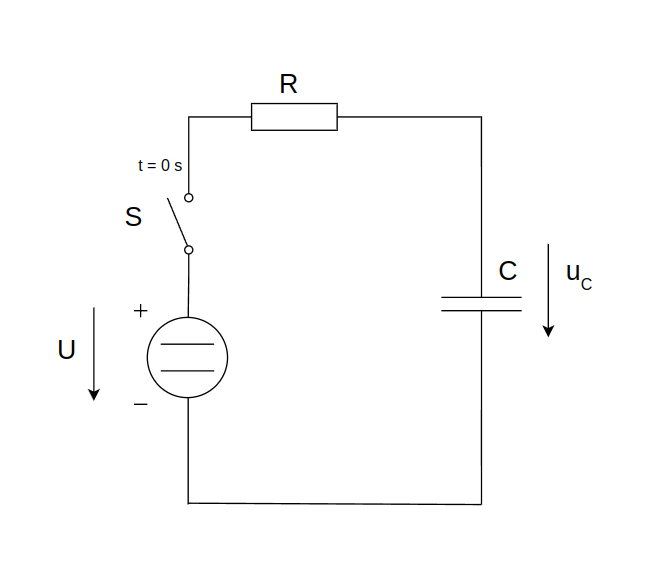
\includegraphics[width=12cm]{priklad5_0}
\centering
\centering
\end{figure}
Známe U, R, C, $U_{C(0)}$\\
1)Ohmův zákon:\\ I = $\frac{U_{R}}{R}$\\
2)Kirchhochův zákon:\\ U = $U_{R}+U_{C}$\\ $U-U_{C}-U_{R}=0$\\
3)Axiom:\\$u_{C}'=\frac{1}{C} \times I$\\ $U_{C}(0)=U_{CP}$\\
1.krok\\
\[
  u_{C}'=\displaystyle\frac{1}{C} \times \displaystyle\frac{1}{R} \times U_{R}
\]
\[
  U_{R} = U-U_{C}
\]
\[
  u_{C}'=\displaystyle\frac{1}{RC} \times (U-u_{C})
\]
Jedná se o diferenciální rovnici 1. řádu\\
\textit{počáteční podmínka:} $u_{C}(0)=U_{CP}$\\
\[
  u_{C}'+\displaystyle\frac{u_{C}}{RC}= \displaystyle\frac{U}{RC}
\]
Charakteristická rovnice:
\[
  \lambda + \displaystyle\frac{1}{RC}=0
\]

\[
  \lambda =-\displaystyle\frac{1}{RC}
\]
Očekávané řešení $u_{C}(t)=K(t)e^{\lambda t} = K(t)e^{-\frac{t}{RC}}$\\
Zderivujeme $u_{c}(t)$:
\[
  u_{c}(t) = K(t)e^{-\frac{t}{RC}}
\]
\[
  u_{c}'(t)=K'(t)e^{-\frac{t}{RC}}- \displaystyle\frac{1}{RC} \times K(t)e^{-\frac{t}{RC}}
\]\\
Nyní $u_{C}(t)$ a $u_{c}'(t)$ dosadíme do $u_{C}'+\frac{u_{C}}{RC}=\frac{U}{RC}$
\[
  K'(t)e^{-\frac{t}{RC}}-\displaystyle\frac{K(t)}{RC}e^{-\frac{t}{RC}}+\displaystyle\frac{K(t)e^{-\frac{t}{RC}}}{RC}=\displaystyle\frac{U}{RC}
\]
\[
  K'(t)e^{-\frac{t}{RC}}=\displaystyle\frac{U}{RC}
\]
Nyní zjistíme K(t)
\[
  K'(t)e^{-\frac{t}{RC}}=\displaystyle\frac{U}{RC}\ /e^{\frac{t}{RC}}
\]
\[
  K'(t)=\displaystyle\frac{U}{RC}e^{\frac{t}{RC}}\ /\int{}{}
\]
\[
  K(t)=\displaystyle\frac{U}{RC}(RCe^{\frac{t}{RC}})
\]
\[
  K(t)=Ue^{\frac{t}{RC}}+k
\]
\textit{k je integrační konstanta}\\

Nyní dosadíme do původní rovnice (TODO:change this text to reflect reality)
\[
  u_{C}(t) = (Ue^{\frac{t}{RC}}+k)e^{-\frac{t}{RC}}
\]
\[
  u_{C}(t)=U+ke^{-\frac{t}{RC}}
\]
Dosadíme $u_{C}(0)=u_{CP}\implies k=0$
\[
  u_{CP}=U+ke^{0}
\]
\[
  u_{CP}-U=k
\]
Analytické řešení
\[
  u_{C}(t) = U + (u_{CP}-U)e^{-\frac{t}{RC}}
\]
Kontrola dosazením hodnot v $u_{C}(0)$
\[
  u_{c}(0) = 20 + (5-20)e^{-\frac{0}{100 \times 8}}
\]
\[
  u_{c}(0) = 20 + (-15)e^{-\frac{0}{800}}
\]
\[
  u_{c}(0) = 20 -15 \times e^{0}
\]
\[
  u_{c}(0) = 5 
\]
\[
  5=5
\]
\end{document}
